\newcommand{\ub}[1]{{bm #1}}

\chapter{Finite differences for Poisson}

\section{Discretization of equations}

When we want to solve a partial differential equation on a computer, we can
typically only do so in an approximate sense, since a computer can only deal
with a finite amount of data. The process of turning a continuous equation into
a finite-dimensional equation suitable for solving on a computer is referred to
as \emph{discretizing} an equation.

There are several ways to go about this, the most popular being \emph{finite
differences}, \emph{finite elements} and \emph{finite volume} discretizations.
Common to all of these approaches is that at the end of the day, the partial
differential equation is turned into a set of linear equations to solve, i.e.
you end up with something on the form
\[
  \bm A \bm u = bm g
\]
where $\bm A$ is the matrix of linear equations, $\bm u$ is the vector of
unknowns we seek and $\bm g$ is the load (the right hand side in the equation
system).

The simplest and least technical of these are the finite difference approach.
Since this is not a course in numerical solution of partial differential
equations, we will focus on this approach only in this course. But most of what
we consider is also applicable to the other forms of discretization due to the
fact that we will mostly focus on the solution of the linear system of
equations.

\section{Finite difference approximations}

\begin{figure}
  \centering
  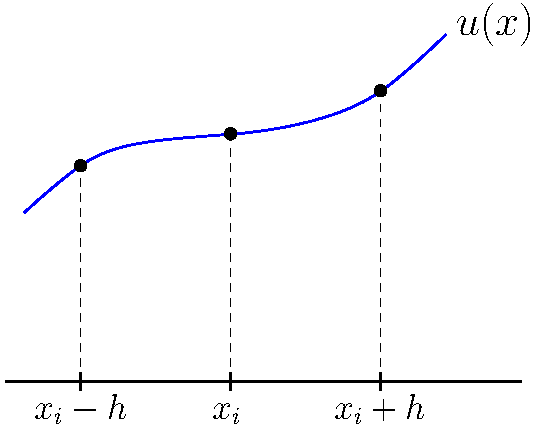
\includegraphics[width=6cm]{FiniteDifference}
  \caption{The function $u(x)$ sampled at a finite difference grid.}
  \label{fig:FiniteDifference}
\end{figure}

Consider the function $u(x)$ depicted in \autoref{fig:FiniteDifference}. A grid
has been introduced---that is, we only consider the function in a discrete sets
of points, $\left\{x_i\right\}_{i=0}^N$, with $x_i = x_0+ih$. Here $h$ is the
grid spacing, here taken as a constant, but in principle we can have a different
spacing between each discrete grid point. We then estimate the derivatives of
this function, only using the values of the function in the discrete sets of
points. This approximation is called a \emph{finite difference}. We now give
alternative finite difference approximations of $u'(x)$ and $u''(x)$ at $x=x_i$.
\begin{align*}
  \intertext{a forward difference approximation:}
  \frac{u(x_i+h)-u(x_i)}{h} &= u'(x_i) + \mathcal{O}(h); \\
  \intertext{two central difference approximations:}
  \frac{u(x_i+h)-u(x_i-h)}{2 h} &= u'(x_i) + \mathcal{O}(h^2), \\ \\
  \frac{u(x_i+h)-2 u(x_i)+u(x_i-h)}{h^2} &= u''(x_i) + \mathcal{O}(h^2).
\end{align*}
The forward difference approximation of $u'(x_i)$ is of first order, meaning
that the error in approximating the first derivative scales linearly with $h$:
if $h$ is reduced by a factor of two, the error is reduced by a factor of two.
The central difference approximations of $u'(x_i)$ and $u''(x_i)$ are of second
order, meaning that the error in approximating the first and second derivatives
scales quadratically with $h$: if $h$ is reduced by a factor of two, the error
is reduced by a factor of four.

We can also generate higher-order approximations to the first and second
derivative of $u(x)$. Higher-order approximations will involve couplings between
more neighboring points.

\section{The one-dimensional Poisson problem}

\subsection{Homogeneous Dirichlet boundary conditions}

We consider here the Poisson equation (or diffusion equation) in one space
dimension,
\begin{align*}
  -u_{xx} = f \qquad \text{in}\,\Omega=(0,1)
\end{align*}
and with homogeneous boundary conditions,
\begin{align*}
  u(0) = u(1) = 0.
\end{align*}

In the following, we will denote the derivative of $u$ with respect to $x$ as
$u_x$, and the second derivative of $u$ with respect to $x$ as $u_{xx}$. This
will prove useful when we later consider two- and three-dimensional problems.

In the Poisson equation, the right hand side $f(x)$ is assumed to be known;
$f(x)$ is often referred to as the source term. In the particular case when
$f=0$, the Poisson equation reduces to the Laplace equation.

In general, the Poisson equation is a partial differential equation (PDE), which
in one space dimension reduces to a standard ordinary differential equation. In
order to obtain a unique solution, we need to specify boundary conditions. In
our case, $u$ is specified at the end points $x=0$ and $x=1$. When $u$ is
specified on the boundary, we say that we have prescribed Dirichlet boundary
conditions. When the prescribed values are zero, as in our case, we say that we
have prescribed homogeneous Dirichlet boundary conditions. The Poisson equation
together with the boundary conditions constitute the Poisson problem.

\begin{figure}
  \centering
  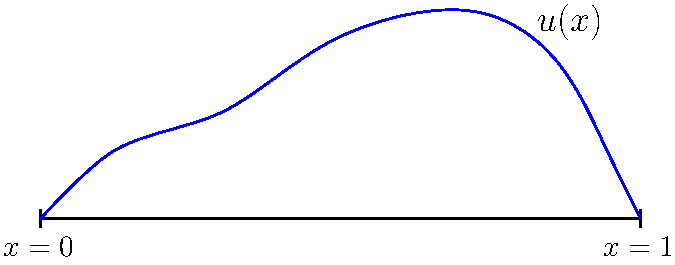
\includegraphics[width=6cm]{Poisson1D_Domain}
  \caption{Domain and solution of the one-dimensional Poisson problem.}
  \label{fig:Poisson1D_Domain}
\end{figure}

\begin{figure}
  \centering
  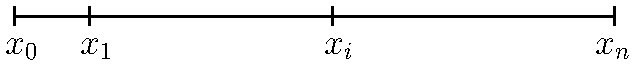
\includegraphics[width=6.5cm]{Poisson1D_Grid}
  \caption{A finite difference grid.}
  \label{fig:Poisson1D_Grid}
\end{figure}

Let $u_i$ be an approximation to $u(x_i)$, $i=1,\ldots,n-1$, and let $f_i =
f(x_i)$. A finite difference approximation of the Poisson problem can then be
expressed as
\begin{align}
  -\left( \frac{u_{i+1} - 2u_i + u_{i-1}}{h^2} \right) &= f_i, \qquad i=1,\ldots,n-1,
  \label{eq:Poisson_int_1d}\\
  u_0 &= 0, \\
  u_{n} &= 0.
\end{align}
We have here $n-1$ unknown values to determine, namely, $u_1, u_2, \ldots,
u_{n-1}$, and we have $n-1$ conditions by requiring that the Poisson equation be
approximated at all the internal grid points $x_1, x_2, \ldots,x_{n-1}$. The
values $u_0$ and $u_{n}$ follow from satisfying the boundary conditions. Note
that we have here used a second order finite difference approximation of
$u_{xx}$.

The equations (\ref{eq:Poisson_int_1d}) can also be expressed as the system
\begin{align*}
  2 u_1 - u_2 &= h^2 f_1, \\
  -u_1 + 2 u_2 - u_3 &= h^2 f_2, \\
  &\vdots \\
  -u_{n-2} + 2 u_{n-1} &= h^2 f_{n-1}.
\end{align*}
We have here already used the fact that $u_0=0$ and $u_{n}=0$.

In matrix form, this system can be expressed as
\begin{align}
 \underbrace{ \begin{pmatrix}
    2 & -1 & & & \\
    -1 & 2 & -1 & & \\
    & & \ddots & & \\
    & & -1 & 2 & -1 \\
    & & & -1 & 2
  \end{pmatrix}
  }_{\bm A}
  \underbrace{ \begin{pmatrix}
    u_1 \\
    u_2 \\
    \vdots \\
    u_{n-2} \\
    u_{n-1}
  \end{pmatrix}
  }_{\bm u}
  &= h^2
  \underbrace{ \begin{pmatrix}
    f_1 \\
    f_2 \\
    \vdots \\
    f_{n-2} \\
    f_{n-1}
  \end{pmatrix}
  }_{\bm f} ,
  \label{eq:A}
\end{align}
or, more succinctly as
\begin{align*}
  \bm A \bm u = \bm g
\end{align*}
where $\bm g = h^2 \bm f$.

It is common to represent the finite difference formula as a stencil, see
\autoref{fig:ThreePointStencil}. By sweeping this across the grid points on our
mesh, it will generate the linear equations given in \eqref{eq:A}.
\begin{figure}
  \centering
  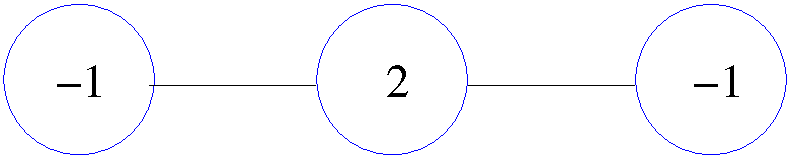
\includegraphics[width=6cm]{ThreePointStencil}
  \caption{
    Weights in the three-point finite difference stencil for the approximation
    of $h^2\cdot$($-u_{xx}$).
  }
  \label{fig:ThreePointStencil}
\end{figure}

We now make some remarks regarding the properties of $\bm A$:
it is a sparse matrix;  more precisely, it is a tridiagonal matrix.
We also note that $\bm A$ is symmetric (i.e., $\bm A = \bm A^\intercal$) and
positive definite (i.e., $\bm v^\intercal \bm A \bm v > 0$ for all vectors $\bm
v \in \mathbb{R}^{n-1}$, $\bm v \not= \bm 0$).

The system of $n-1$ equations is solvable and has a unique solution
\[
  \bm u = \begin{pmatrix} u_1 & u_2 & \cdots & u_{n-1} \end{pmatrix}^\intercal.
\]

The error at the grid points is of second order, i.e.
$|u(x_i)-u_i| \sim \mathcal{O}(h^2)$.

\subsection{Nonhomogeneous Dirichlet boundary conditions}

If $u_0, u_{n} \not= 0$, we can write the $n-1$ equations
\eqref{eq:Poisson_int_1d} as
\begin{align}
  \begin{pmatrix}
    2 & -1 & & & \\
    -1 & 2 & -1 & & \\
    & & \ddots & & \\
    & & -1 & 2 & -1 \\
    & & & -1 & 2
  \end{pmatrix}
  \begin{pmatrix}
    u_1 \\
    u_2 \\
    \vdots \\
    u_{n-2} \\
    u_{n-1}
  \end{pmatrix}
  &= h^2
  \begin{pmatrix}
    f_1 \\
    f_2 \\
    \vdots \\
    f_{n-2} \\
    f_{n-1}
  \end{pmatrix}
  +
  \underbrace{ \begin{pmatrix}
    u_0 \\
    0 \\
    \vdots \\
    0 \\
    u_{n}
  \end{pmatrix}
  }_{\bm b}.
  \label{eq:Poisson1D_DirBC}
\end{align}
This system can again be expressed on the form
\begin{align*}
  \bm A \bm u = \bm g,
\end{align*}
where the left hand side is the same as before. However, the right hand side is
now $\bm g = h^2 \bm f + \bm b$, where the additional vector $\bm b$ is defined
in \eqref{eq:Poisson1D_DirBC}.

\section{Two-dimensional Poisson problem}

We now consider the Poisson problem in a rectangular domain with lengths $L_x$
and $L_y$; see \autoref{fig:Poisson2D_Domain}. The Poisson problem we consider
can be expressed as
\begin{alignat*}{2}
  -\nabla^2 u &= f & \qquad &\text{in}\, \Omega, \\
  u &= 0 & \qquad & \text{on}\, \partial \Omega.
\end{alignat*}
where the right hand side $f(x,y)$ (the source term) is assumed to be known.

\begin{figure}
  \centering
  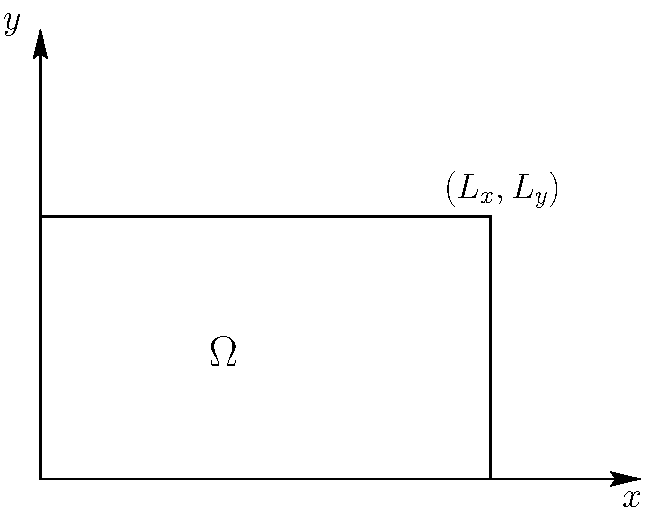
\includegraphics[width=6cm]{Poisson2D_Domain}
  \caption{A rectangular domain for the two-dimensional Poisson problem.}
  \label{fig:Poisson2D_Domain}
\end{figure}

\begin{figure}
  \centering
  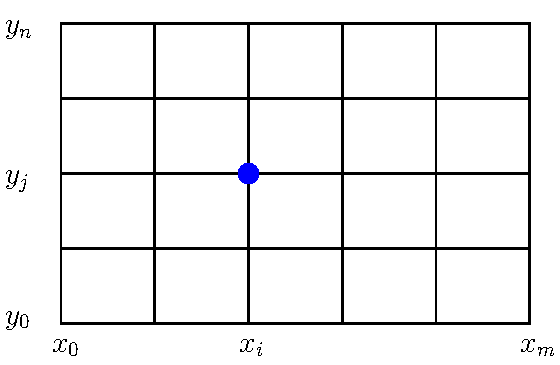
\includegraphics[width=7cm]{Poisson2D_Grid}
  \caption{Finite difference grid: a structured grid.}
  \label{fig:Poisson2D_Grid}
\end{figure}

\subsection{Finite difference discretization}

The finite difference grid points (or nodes) in \autoref{fig:Poisson2D_Grid} are
given by
\begin{align*}
  x_i &= i \cdot h_x, \quad i=0,1,\ldots,m, \qquad h_x = \frac{L_x}{m}, \\
  y_j &= j \cdot h_y, \quad j=0,1,\ldots,n, \qquad h_y = \frac{L_y}{n}.
\end{align*}
Let $u_{i,j}$ be an approximation to $u(x_i,y_j)$, $1\leq i\leq m-1$, $1\leq
j\leq n-1$, and let $f_{i,j} = f(x_i,y_j)$. Then
\begin{align*}
  \frac{u_{i+1,j} - 2 u_{i,j} + u_{i-1,j}}{h_x^2}
  &\simeq \left( \frac{\partial^2 u}{\partial x^2} \right) \biggl|_{(x_i,y_j)} + \mathcal{O}(h_x^2), \\
  \frac{u_{i,j+1} - 2 u_{i,j} + u_{i,j-1}}{h_y^2}
  &\simeq \left( \frac{\partial^2 u}{\partial y^2} \right) \biggl|_{(x_i,y_j)} + \mathcal{O}(h_y^2).
\end{align*}

Assuming (for simplicity) that $m=n$, and that $h_x=h_y=h$, the approximation of
the Poisson problem at the internal grid points can be expressed as
\begin{align*}
  -\frac{(u_{i+1,j}-2u_{i,j}+u_{i-1,j})}{h^2}
  -\frac{(u_{i,j+1}-2u_{i,j}+u_{i,j-1})}{h^2}
  &= f_{i,j}, \qquad i,j=1,\ldots,n-1,
\end{align*}
or
\begin{align}
  -u_{i+1,j}-u_{i-1,j}-u_{i,j+1}-u_{i,j-1}+4u_{i,j} &= h^2 f_{i,j}, \qquad i,j=1,\ldots,n-1.
  \label{eq:Poisson2D_disc}
\end{align}
We note that each unknown value $u_{i,j}$ is coupled to its nearest neighbors
(north, south, east, west) according to the five-point stencil we are using; see
\autoref{fig:FivePointStencil}.

\begin{figure}
  \centering
  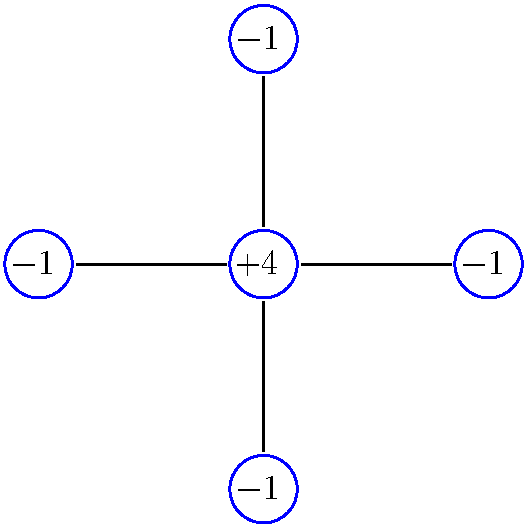
\includegraphics[width=6cm]{FivePointStencil}
  \caption{
    Weights in the five-point finite difference stencil for the approximation of
    $h^2\cdot$($-\nabla^2$).
  }
  \label{fig:FivePointStencil}
\end{figure}

\subsection{Global numbering scheme}

In order to generate a matrix system as in the one-dimensional case, we need to
define a unique ordering of all the degrees-of-freedom. We will here use a
``natural'' ordering in the sense that we number the \emph{internal} nodes along
the $x$-direction first, i.e.
\begin{align*}
  u_{k=(n-1)(j-1)+i} & \equiv u_{i,j} \\
  f_{k=(n-1)(j-1)+i} &\equiv f_{i,j}
\end{align*}
Here, $k = 1,\ldots,N$ with $N=(n-1)^2$. We see that the ordering maps each
node, $(i,j)$, in the grid to a unique, global index, $k$; see
\autoref{fig:NaturalOrdering}.

\begin{figure}
  \centering
  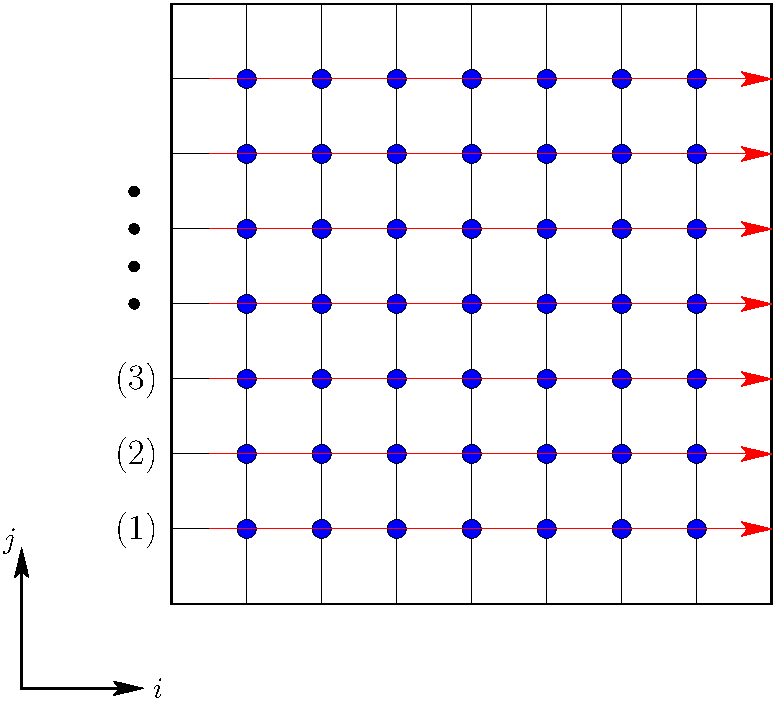
\includegraphics[width=7cm]{NaturalOrdering}
  \caption{
    We use a ``natural'' ordering of the unknowns: we first number all the
    \emph{internal} nodes along ``row'' 1 (in the $x$-direction), followed by
    the nodes in ``row'' 2, etc. The boundary nodes are not counted since these
    values are assumed to be known.
  }
  \label{fig:NaturalOrdering}
\end{figure}

\subsection{System of equations}

With the chosen numbering scheme of the unknowns, we can express the discrete
equations \autoref{eq:Poisson2D_disc} as
\begin{align}
  \bm A \bm u = \bm g,
  \label{eq:Poisson2D_sys}
\end{align}
where the matrix $\underline{A}$ and the vectors $\bm u$ and
$\bm g$ are defined in \autoref{fig:Poisson2D_sys}. The dimension of
this system is $N=(n-1)^2$. The matrix $\bm A$ is still sparse; in particular,
it is pentadiagonal, reflecting the use of a five-point stencil for the
approximation of the Laplace operator. However, while the bandwidth in the
one-dimensional case is one, the bandwidth is now $n$.

Finally, we remark that the matrix $\bm A$ is symmetric and positive definite as
in the one-dimensional case. This will guarantee that the system
\eqref{eq:Poisson2D_sys} is solvable and will yield a unique solution
$\bm u = \begin{pmatrix}u_1&\cdots&u_N\end{pmatrix}^\intercal$. The
discretization error is still quadratic in the grid spacing $h$,
\begin{align*}
  |u(x_i,y_j)-u_{i,j}| \sim \mathcal{O}(h^2). \\
\end{align*}

\begin{figure}
  \centering
  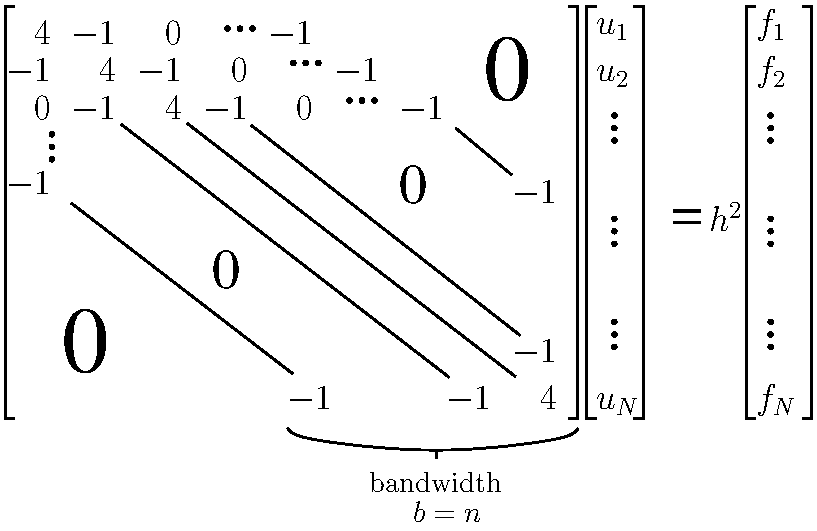
\includegraphics[width=8.5cm]{Poisson2D_System}
  \caption{
    The system of algebraic equations following from the discretization of the
    two-dimensional Poisson problem in a rectangle, and using a ``natural''
    ordering system for the unknowns.
  }
  \label{fig:Poisson2D_sys}
\end{figure}

\subsection{Solution methods for $\bm A \bm u = \bm g$}

Once we have generated the system of equations $\bm A \bm u = \bm g$, we need to
solve this system. There are two main classes of solution methods: direct and
iterative methods. We now give a brief discussion of each of these classes.

\subsubsection{Direct methods}

A direct solution method is method which solves the system of algebraic
equations in a finite, predictable number of steps, e.g., Gaussian elimination,
FFT, etc. This class of the solution methods is often robust, especially when
$\bm A$ is symmetric and positive definite.

In the following, we will use the following notation:
\begin{align*}
  \mathcal{N}_\text{op} &= \text{number of floating-point operations} \\
  \mathcal{M} &= \text{memory requirement (in number of bytes)}
\end{align*}

We will also assume that $\bm A \in \mathbb{R}^{N \times N}$.

As an example, consider full LU-factorization (Gaussian elimination). In this
case, we do not exploit any information about sparsity of $\underline{A}$, but
treat this as a full matrix. For this solution approach, we have
\begin{align*}
  \mathcal{N}_\text{op} &\sim \mathcal{O}(N^3), \\
  \mathcal{M} &\sim \mathcal{O}(N^2).
\end{align*}
Full LU-factorization is robust and easy to use, however the cost does not scale
very well since we need $\mathcal{O}(N^2)$ operations per unknown. For large
systems, this cost becomes prohibitive.

A better approach is to exploit the banded structure of $\bm A$; see
\autoref{fig:Banded}. For a banded LU-factorization, we have
\begin{align*}
  \mathcal{N}_\text{op} &\sim \mathcal{O}(N b^2) ,\\
  \mathcal{M} &\sim \mathcal{O}(N b) .
\end{align*}

\begin{figure}
  \centering
  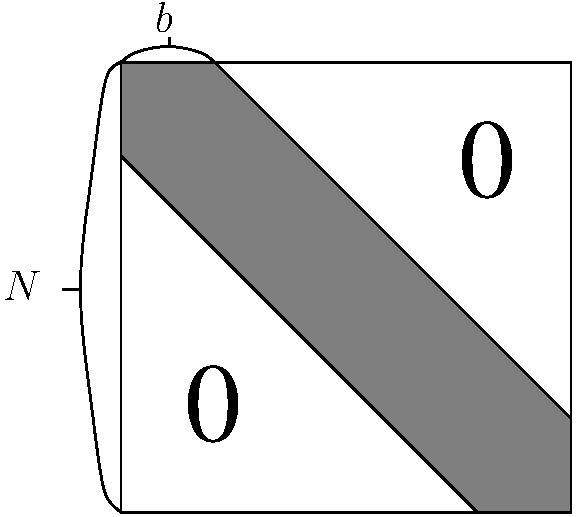
\includegraphics[width=6cm]{BandedMatrix}
  \caption{
    A banded matrix with band width $b$. In the context of solving partial
    differential equations numerically, we often have $b \ll N$.
  }
  \label{fig:Banded}
\end{figure}

We remark that, since $\bm A$ is symmetric and positive definite, no pivoting is
necessary during the Gaussian elimination process.

\begin{figure}
  \centering
  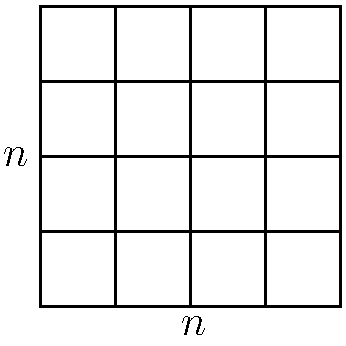
\includegraphics[width=4cm]{Poisson2D_ntimesnGrid}
  \caption{
    The two-dimensional grid associated with the finite difference solution of
    the Poisson problem. Here, $N \sim n^2$, while the bandwidth of
    $\bm A$ using a natural numbering scheme is $b\sim n$.
  }
  \label{fig:Poisson_nxn}
\end{figure}

Let us now revisit \eqref{eq:Poisson2D_sys} which we arrived at based on a
finite difference discretization of the two-dimensional Poisson problem. If we
exploit the banded structure of $\bm A$ during the LU-factorization, see
\autoref{fig:Poisson_nxn}, the cost of this method is
\begin{align*}
  \mathcal{N}_\text{op} &\sim \mathcal{O}(N b^2)
                          \sim \mathcal{O}(n^4) \sim \mathcal{O}(N^2)\\
  \mathcal{M} &\sim \mathcal{O}(N b) \sim \mathcal{O}(n^3) \sim \mathcal{O}(N^{3/2})
\end{align*}

However, if we instead use FFT (The Fast Fourier Transform), as we will discuss
later, the cost of solving \eqref{eq:Poisson2D_sys} is only
\begin{align*}
  \mathcal{N}_{op} &\sim \mathcal{O}(N \log N), \\
  \mathcal{M} &\sim \mathcal{O}(N).
\end{align*}
This is approximately optimal since the computational cost is $\mathcal{O}(\log
N)$ per unknown, and the memory requirement is constant per unknown, independent
of the value of $N$.

\subsubsection{Iterative methods}

An iterative method will give a new estimate or update of the solution at each
iteration. In most cases, the exact solution to $\bm A \bm u = \bm g$ will never
be reached. However, one can get as close as one wishes, but this may require
many iterations and imply a high computational cost. Unlike a direct method, the
solution is not reached after a finite, predictable number of floating point
operations. In order to stop the iteration, a stop criterion has to be specified
by the user. This can be some kind of tolerance, e.g. that the residual (i.e.
the difference between the left hand side and the right hand side of the
equation system) is less than a tolerance. Typically, when the tolerance is
reduced, the number of iterations increases.

Another aspect with iterative methods is that the computational cost can be
problem dependent; see \autoref{fig:Poisson_aspect}. This is different from
direct solution methods which often only depends on the problem size, $N$.

\begin{figure}[!ht]
  \centering
  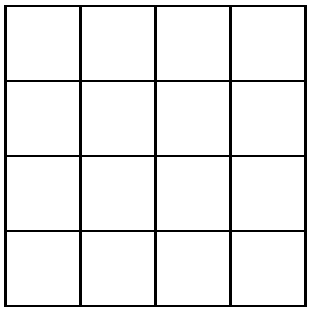
\includegraphics[height=0.2\textwidth]{Poisson2D_aspect1} \\
  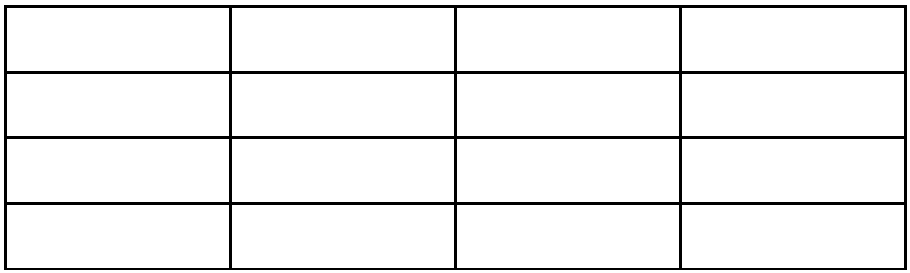
\includegraphics[height=0.2\textwidth]{Poisson2D_aspect2}
  \caption{
    Two different computational domains for the Poisson problem, but with the
    same number of unknowns after discretization. The problem size, $N$, is
    therefore the same. The number of iterations required to solve the system of
    algebraic equations will depend on the aspect ratio (the ratio $L_x/L_y$) of
    the domains. Hence, the computational cost for solving the problem on the
    right will be higher than for the problem on the left. This is in contrast
    to a direct method where the computational cost for solving the two systems
    will be the same.
  }
  \label{fig:Poisson_aspect}
\end{figure}

A great advantage of many iterative methods is that they often have a
\emph{scalable} memory requirement, i.e. that the memory requirement is
proportional to $N$ and not some power of $N$.

Another characteristics with iterative methods is that much of the computational
cost is related to performing basic linear algebra operations such as
matrix-vector products, inner products, etc.

Finally, we remark that iterative methods are very suitable for parallel
processing, and are often the only viable alternative for large,
three-dimensional problems.

Some examples of iterations methods suitable for symmetric and positive definite
problems are: Jacobi iteration, Gauss-Seidel iteration, the conjugate gradient
method, and multigrid methods (where the last two methods are commonly used
today).
